\chapter{Different Approaches for Proofs to Demonstrate Turing Completeness}\label{chapter:ProofApproachesForTC}

\section{Overview}\label{sec:ProofOverview}

We will be exploring the different approaches to demonstrate TC for different systems.
I have outlined the approaches based on their respective discipline, increasing in abstraction.
With each discipline comes a more theoretical view and understanding of TMs and TC systems.
My intention is to add clarity on the logic for these proofs/techniques.
For example, in the Computer Engineering perspective, TM is created from its mechanical properties through the usage of logic gates.
This is vastly different compared to how Mathematicians show TC, which is through the use of Lambda calculus -- a model for representing mathematical logic.
All proofs are equivalent in goal, however.
These are not the only perspectives and types of proofs for showing Turing Completeness as well as TMs.
This is simply a survey into what TMs and Turing Completeness looks like across the disciplines.

\section{Computer Engineering}\label{sec:CE}

In this section, we will analyze what a TM looks like from a physical perspective.
This may seem contradictory because the TM is described as a theoeretical machine.
But in fact, the very computers that we use today are are capable of processing TC systems through the usage of programming languages.
This means that they are limited TMs, because they are bounded only in memory.
In this approach, we will look at the core components of Computer Engineering to create a TM.

\subsection{Logical Design of a TM}\label{subsec:TMLogicalDesign}

To define what a TM does, we must explore what it is capable of.
Recall Theorem \ref{thm:CTT} in section \ref{subsec:Church-Turing Thesis}, "Every effectively calculable function can be computed by a Turing Machine."
Every effectively calculable function, as Turing and Church understood, was any mathematical calculation.
This means that a TM must have some ability to perform any operation on numbers, such as the basic operations of addition, subtraction, multiplication, and division.
Furthermore, they must be capable of combining these together to form more complex operations such as exponential arithmetic.
Beyond the mathematical aspect, they must allow for logical processing \cite{ChemTM}.

\subsubsection{Architecture}\label{subsubsec:Arch}

Looking at modern day computer architecture, there are several components that work independently but operate concurrently.
It is based off of the Modified Harvard Structure which is a variation of the Harvard computer architecture and Von Neumann architecture.
It combines both approaches towards computer architecture to handle many tasks that were difficult to handle using one of either architecture.

The von Neumann Architecture which has a centralized CPU to handle tasks for the computer.
All processes are handled by the CPU directly.
It contains several parts inside for processing data.
Inside the CPU is an ALU with registers, as well as a Control Unit.
The ALU processes arithmetic and logical computation, with the assistance of registers to store data at each step.
The Control unit determines the commands to be given to the ALU and other parts of the computer.
There is an associated Memory Unit which is where the bulk of memory storage lies.
Outside of the CPU are the Input and Output devices \cite{vonNeumannBook}.

\begin{figure}[htb]
    \centering
    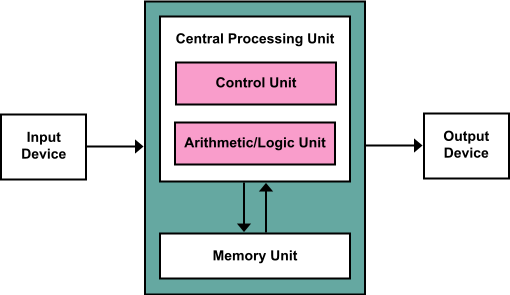
\includegraphics[width=10cm]{Images/Von_Neumann_Architecture.png}
       \caption{Von Neumann architecture \cite{vonNeumannImg}.}
           \label{fig:VonNeumannArch}
\end{figure}

Figure \ref{fig:VonNeumannArch} visually describes the architecture \cite{vonNeumannImg}.
The von Neumann architecture has several limitations, with one of the biggest criticisms being that it is bottlenecked by the throughput between the CPU and memory.
Essentially, the CPU will eventually have more processing power than the bus can handle to write/read from memory.
This causes the CPU to wait until the bus is freed to continue processing.
As an alternative, we will now look at the Harvard Architecture

The Harvard architecture looks at the problem as says that if the CPU is too large and complex, then each individual component should be separated.
This allows for the tasks to be distributed evenly amongst the several smaller components like the ALU and Instruction memory as opposed to having them live inside the CPU.
The CPU is capable of simultaneous reads and writes.
However, a similar bottleneck occurs where the bus connecting each of the components is the limiting factor.
Figure \ref{fig:HarvardArch} illustrates the Harvard Architecture \cite{HarvardArchImg}.

\begin{figure}[htb]
    \centering
    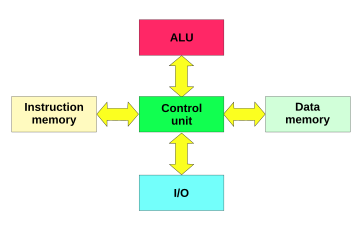
\includegraphics[width=10cm]{Images/Harvard_architecture.svg.png}
       \caption{Harvard architecture \cite{HarvardArchImg}.}
           \label{fig:HarvardArch}
\end{figure}

However, modern day computers utilize a mixed computer architecture called the Modified Harvard architecture.
It combines both architectures into a single model.
This usually is of the form of separating the components of the computer, but allowing several smaller memory caches for the CPU.
This is why modern computers utilize several components such as the CPU, GPU, Main Memory (SDD or HDD) and so forth.
Furthermore, this advancement allows for paralellism or multi-core systems to arise.
Some notable examples include the NVIDIA RTX 4080 which has over 8000 cores or for the intel i9-13900ks CPU to have 16 cores \cite{4080Specs,IntelSpecs}.
By allowing each one to independently operate, but still have the CPU as the "brains" of the operation.
We will now dive slightly deeper into the discussion to see what lies beneath these components within modern computer systems.

\subsubsection{Logic Gates}\label{subsec:LogicGates}

The basic building blocks for devices such as the ALU, CPU, and such are logic gates.
These are simplistic logical components that allow for processing of data and performing operations on them.

The core of the CPU relies on the ALU.
This is because the CPU determines what operations to perform on what data.
The ALU then receives the command to perform some arithmetic logic, and returns the result.
The ALU contains registers which hold the temporary data for calculations.
Eg. the multi-step operation $(2 * 4) + 1$ requires several cycles and the ability to store the intermediary step $(2 * 4)$ without sending it as the result.
These smaller registers are associated with an address for referencing purposes, and are not seen by the CPU.
Instead the CPU manages it's own memory with caches and main memory.

Within the ALU there are smallers components that perform specific operations such as addition and subtraction.
These smaller components utilize logical gates such as the OR gate to compute the result with the given input.
Figure \ref{fig:2BitALUSimp} describes a highly simplistic view of what a 2-Bit ALU may look like \cite{SimpleALU}.

\begin{figure}[htb]
    \centering
    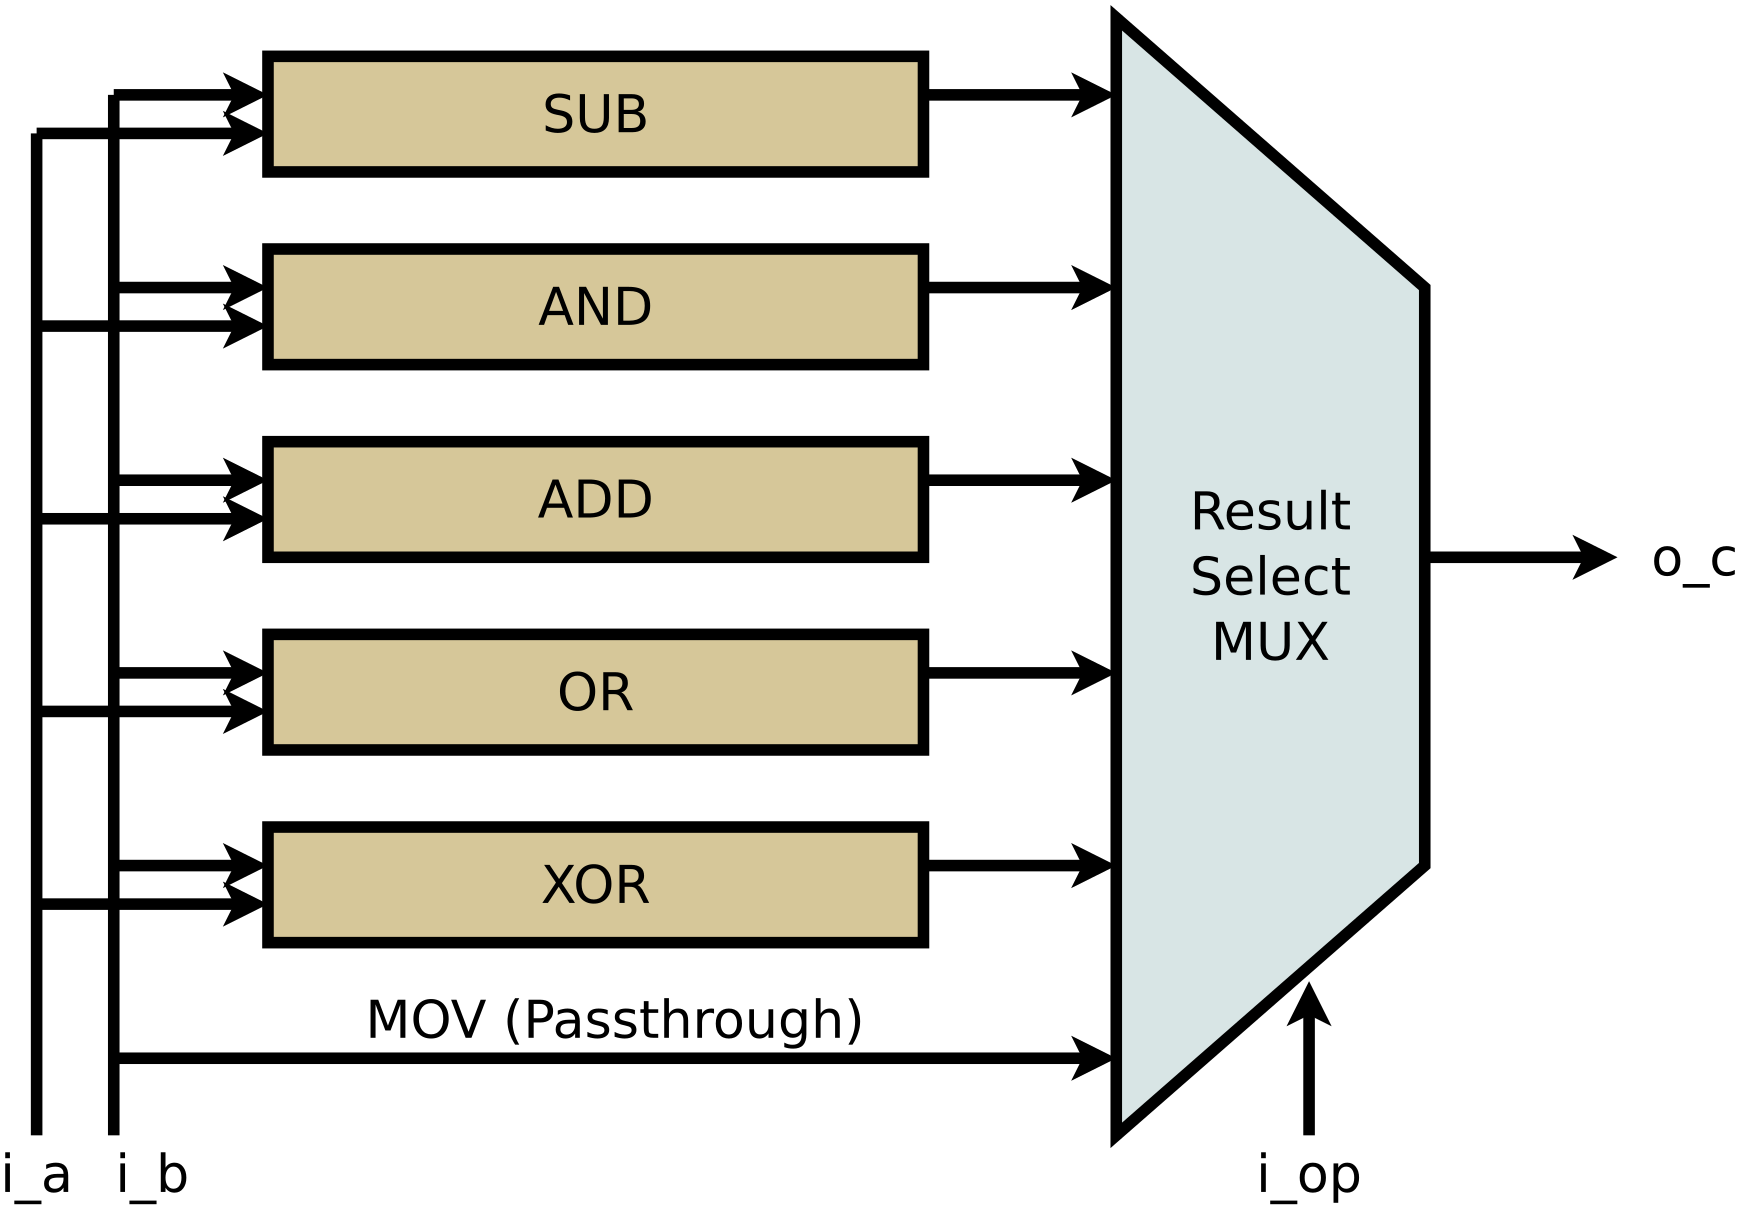
\includegraphics[width=10cm]{Images/alu-simple.png}
       \caption{A 2-Bit ALU \cite{SimpleALU}.}
           \label{fig:2BitALUSimp}
\end{figure}

It accepts two inputs, $i_a$ and $i_b$ which are the inputs to the given operation.
These inputs are fed into the respective operation handler, SUBtract, AND, ADDition, OR, XOR, or MOVe.
The operation handles these inputs and uses the logical gates to perform the desired operation.
This result then gets sent to the MUX which will also take in the operation $i_{op}$ and only accept the output from the desired operation.
This result is then output as $o_c$.

This simplistic design lacks the ability to handle multi-step operations.
It also lacks the actual layout of the ADD or OR operations.
It instead abstracts them to display the circuit in a more digestible manner.
As such, I have provided a more in-depth version of an ALU which lacks many of the operations seen in Figure \ref{fig:2BitALUSimp}.
It explicitly shows the physical design of a different ALU \cite{ALUImg}.

\begin{figure}[htb]
    \centering
    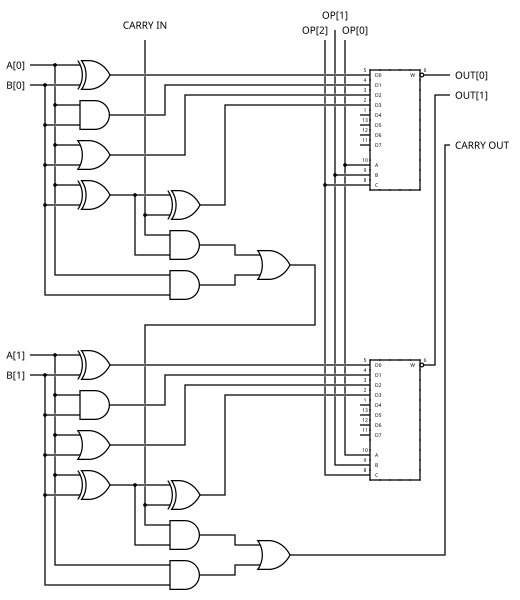
\includegraphics[width=10cm]{Images/2-bit_ALU.svg.png}
       \caption{A 2-Bit ALU \cite{ALUImg}.}
           \label{fig:2BitALUAdv}
\end{figure}

Figure \ref{fig:2BitALUAdv} only has 3 operations: OR, AND, XOR.
The inputs are labeled $A$ and $B$ with the operation defined as $OP[1], OP[2], OP[3]$.
$A[0]$ refers to the least-significant bit of $A$ while $A[1]$ refers to the most-significant bit.
These inputs are fed to all operation sequences (OR, AND, XOR), and sent to both the top and bottom MUX.
These MUX then output the desired result from the $OP[NUMBER]$ desired as $OUT[0]$ and $OUT[1]$.

Overall, by combining these circuits together, one can create more powerful mechanisms like ADD, MUX, etc.
To construct a physical TM using such circuitry, assuming unbounded memory amongst other conditions, seems possible.

\subsection{Constructing the TM}\label{subsec:CreateTM}

With the ability to construct logic gates, we can create more complex components such as the ALU, which would be used within the CPU, and overall create the computer from the bottom-up.
Accompanied with the ability to store memory, as well as have a way to interact with the system through Input and Output, it is possible to create a functional computer.
Developers have successfully created computers in the well-known video games of Minecraft and Terraria respectively in \cite{MCTM,TerrariaTM,TerrariaTMGH}.
In fact, I will discuss a method to demonstrate TC that verifies that the computer built inside Terraria is verifiably TC via a method discussed in \ref{subsubsec:CGoL}.

This means that to construct a TM on a physical level (of course alleviating the restriction of unbounded memory), these would be the minimum requirements \cite{nand2tetris,ELTCompSys}:
\begin{itemize}
    \item ADD
    \item SUB
    \item MUX
    \item OR
    \item AND
    \item XOR
\end{itemize}

Which themselves rely on logic gates as building blocks.
Therefore, if it is possible to create simulate logic gates, or to create the above shown processes, then it is capable of satisfying any arithmetic or logical calculation.
As such, the Church-Turing Thesis, Theorem \ref{thm:CTT}, is met and a TM can be created.

\section{Computer Science}\label{sec:CompSci}

In this section, I will conceptualize what a TM looks like under the lens of Computer Science.
There are 2 main perspectives: that of Automata Theory and the Software Engineering approach.
The Automata Theory approach utilizes theoretical designs based off of those utilized by Turing and Gavin.
The Software Engineering approach instead applies it to a problem to showcase Turing Completeness via programming with code.

\subsection{Automata Theory}\label{subsec:AutomataThy}

I will now abstract from the physical understanding of how to create a TM, to creating a theoretical one using Automata theory.
In automata theory, Turing Machines are described using logical notation.
The definition of a TM has several interpretations, but I will outline a slightly more advanced description \cite{IntroFormLangAuto,TuBB}.
The illustrated TM allows for the machine to stay at the current cell.

\begin{definition}
    \label{def:TM}
    A Turing Machine $M$ is defined by:
        \[M = (Q, \Sigma ,\Gamma, \delta, q_{0}, \raisebox{0.1cm}{\fbox{}}, F)\]
        \par \hangindent=3cm \hangafter=1
        where: \\
        \( Q \) is the set of internal states,\\
        \( \Sigma \) is the input alphabet,\\
        \( \Gamma \) is the finite set of symbols called the tape alphabet,\\
        \( \delta \) is the transition function,\\
        \( \raisebox{0.1cm}{\fbox{}} \in \Gamma \) is a special symbol called the blank,\\
        \( q_{0} \in Q \) is the initial state,\\
        \( F \subseteq Q \) is the set of final states.
\end{definition}

The transition function $\delta$ is defined as \[\delta: Q \times \Gamma \rightarrow Q \times \Gamma \times \{L, R, S\}.\]
This means that for a given $\delta$ transition with inputs $q \in Q$ and $a \in \Gamma$, the tape will move to another state $x \in Q$, clear the current cell (indicated by \raisebox{0.1cm}{\fbox{}}) or some symbol $y \in \Gamma$, and choose to move the tape head Left one cell (L), Right one cell (R), or to Stay at the current cell (S).
An example transition can be written: \[\delta(q_{0}, a) = (q_{1}, d, R)\] where the internal state is $q_{0}$, and we read input token a.
After the transition, we have internal state $q_{1}$, wrote symbol d onto the tape, and moved to the right one cell.
See Figure \ref{fig:DeltaTransition} demonstrating this change:

\begin{figure}[htb]
    \centering
    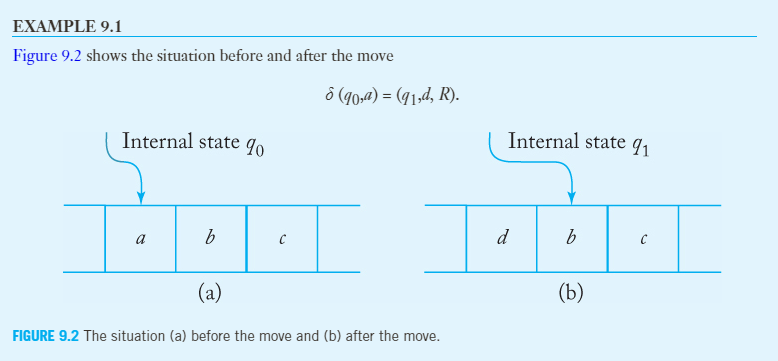
\includegraphics[width=16cm]{Images/deltatransition.png}
       \caption{Delta transition example from \cite{IntroFormLangAuto}.}
           \label{fig:DeltaTransition}
\end{figure}

Recall Figure \ref{fig:TM} which represents a simplistic TM.
In formal nomenclature, it can be written as follows:
\[
    \begin{aligned}
        Q &= \{q_{0}, q_{1}, q_{2}\} \text{ with associated labels \{Even, Odd, Halt\}}\\
        \Sigma &= {0,1}\\
        \Gamma &= {0,1}\\
        F &= \{q_{2}\}\\
        q_{0} &\in \text{ Q as the initial state}
    \end{aligned}
\]
and
\[
    \begin{aligned}
        \delta (q_{0}, 0) &= (q_{2}, 1, S),\\
        \delta (q_{0}, 1) &= (q_{1}, \raisebox{0.1cm}{\fbox{}}, R),\\
        \delta (q_{1}, 0) &= (q_{2}, 0, S),\\
        \delta (q_{1}, 1) &= (q_{0}, \raisebox{0.1cm}{\fbox{}}, R).\\
    \end{aligned}
\]

\subsubsection{Notable examples using Formal language}\label{subsubsec:NotableEgsFormalLang}

The proofs constructed using formal language usually modify the given system to meet these requirements.
They must first demonstrate that the input to the system is Undecidable or able to reduced to the Halting problem.
Furthermore, they must create a TM using the system to demonstrate that it is capable of calculating anything.

(EN - I can explain deeper how they work in this section, but it is pretty complex and so i avoid that by briefly describing them)

In "Magic: the Gathering is Turing Complete", the authors modified the way the game is understood between 2 players.
They make the system force moves through clever leverage of the cards and their functions within the game \cite{MtGTC}.

In a different paper, "Turing Completeness and Sid Meier's Civilization", the system was also creatively modified to demonstrate Turing Completeness.
In each game, they constructed UTMs by utilizing the layout of the maps, as well as mechanics for changing states of the roads within the game \cite{CivTC}.

To show that Java Generics are TC, the authors showed that by creating a subtyping machine, it corresponds to only a small portion of the Java Generics while simulating TMs.
Following this discovery, they simulate a TM and then show that the given inputs are undecidable \cite{JavaGenericsTC}; leveraging an extension of Rice's Theorem, Theorem \ref{thm:RiceThm}.

The idea of describing the system as a TM and showing it has an undecidable input is a common practice.
This technique is also seen in a paper titled "The Game Description Language is Turing Complete" \cite{GDLTC}.

\subsection{Software Implementation}\label{subsec:SoftwareImplementation}

As opposed to the various theoretical approaches seen previously in section \ref{subsec:AutomataThy}, this section outlines a different perspective.
Instead of constructing a TM within the compounds of the system, an equivalent proof is to implement a program that demonstrates TC.
By implementing any known TC program successfully implies that the overall system is TC.
For example, the popular Sony PlayStation game "LittleBigPlanet" released for the PlayStation 3, is TC as shown by someone implementing Conway's Game of Life inside of it \cite{LittleBigCGoL}.

One such implementation would be to create a functional example of a known TC cellular automata.
Cellular automata are models of computation which use grids of cells.
Each cell contains a finite number of states, belonging to only one at any given time.
There are rules that determine what state a cell should become.
These rules are applied to all cells simultaneously, and thus form the next step in the sequence.
These steps are made sequentially to show the changes over time.
This makes all cellular automata 0-player games, meaning after an initial configuration there is no further input from the user.
With the work from Stephen Wolfram and other researchers such as Matthew Cook, some of these rules of cellular automata have been shown to be TC.
Famous examples of cellular automata include Conway's Game of Life, Rule 110, and Langton's Ant \cite{CellAutWiki,CellAutWolfram,CGolTM,AntyParticles,AntWiki}.

Cellular automata are sorted into 4 classes:
\begin{itemize}[leftmargin=2cm]
    \item Class 1: Nearly all initial patterns evolve quickly into a stable, homogenous state.
    Any randomness in the initial pattern disappears.
    \item Class 2: Nearly all initial patterns evolve quickly into stable or oscillating structures.
    Some of the randomness in the initial pattern may filter out, but some remains.
    Local changes to the initial pattern tend to remain local.
    \item Class 3: Nearly all initial patterns evolve in a pseudo-random or chaotic manner.
    Any stable structures that appear are quickly destroyed by the surrounding noise.
    Local changes to the initial pattern tend to spread infinitely.
    \item Class 4: Nearly all initial patterns evolve into structures that interact in complex and interesting ways, with the formation of local structures that are able to survive for long periods of time.
    Class 2 type stable or oscillating structures may be the eventual outcome, but the number of required to reach this state may be very large, even when the initial pattern is realtively simple.
    Local changes to the initial pattern may spread indefinitely.
\end{itemize}

Wolfram conjectured that many class 4 cellular automata are capable of universal computation.
Both Conway's Game of Life and Rule 110 exhibit "Class 4 behavior" and have been proven to be Turing Complete \cite{CGoLTM,CellAutBook}.

\subsubsection{Conway's Game of Life}\label{subsubsec:CGoL}

Conway's Game of Life is a 2D grid of cells extending infinitely in the cartesian plane.
Each cell may switch between only 2 states: Alive (On) or Dead (Off).
The rules of CGoL are simple and are illustrated in Figure \ref{fig:cgolrules} \cite{CGoLImg}.
CGoL is considered undecidable.
This is because given any initial pattern and a desired pattern at some later generation, there is no algorithm to determine whether the desired pattern will exist.
As such, it is analogous to the Halting Problem.

\begin{enumerate}
    \item Any live cell with fewer than two live neighbors dies. (Underpopulation)
    \item Any live cell with two or three live neighbors lives on to the next generation. (Survival)
    \item Any live cell with more than three live neighbors dies. (Overpopulation)
    \item Any dead cell with exactly three live neighbors becomes a live cell. (Reproduction)
\end{enumerate}

\begin{figure}[h!]
    \centering
    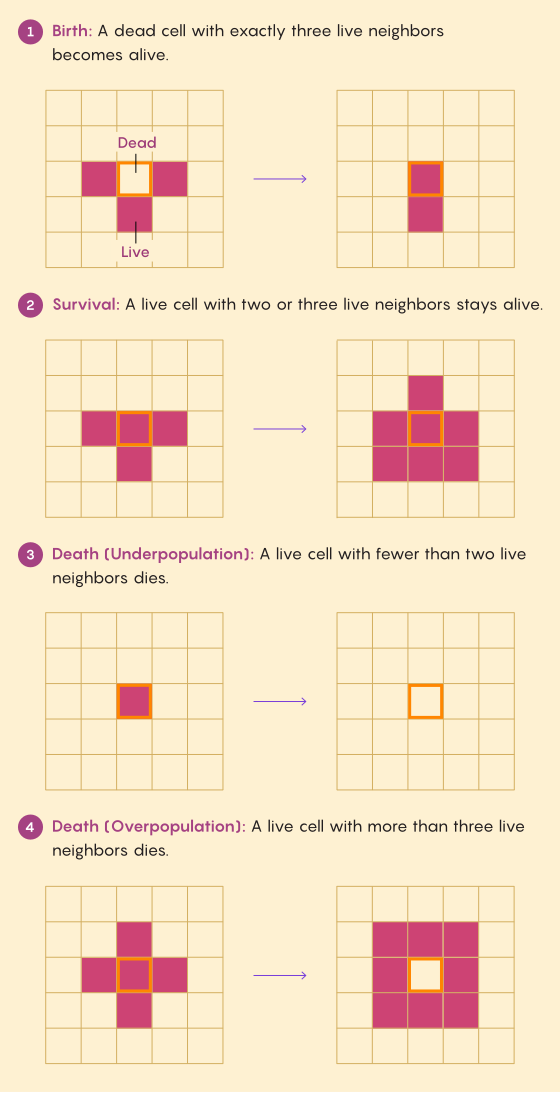
\includegraphics[width=10cm]{Images/CGoL.png}
       \caption{Rules of Conway's Game of Life visualized \cite{CGoLImg}.}
            \label{fig:cgolrules}
\end{figure}

\newpage

\subsubsection{Rule 110}\label{subsubsec:Rule110}

Whereas CGoL is created on a 2D plane, Rule 110 lives in the 1D space.
There is an infinite tape of cells that each may exist in one of two states: 0 or 1.
By looking at three cells in series, one can find what the next state of the middle cell will be.
Below are the rules for Rule 110 with an associated graphic in Figure \ref{fig:Rule110} \cite{Rule110Img}:

\begin{enumerate}
    \item 111 makes 0
    \item 110 makes 1
    \item 101 makes 1
    \item 100 makes 0
    \item 011 makes 1
    \item 010 makes 1
    \item 001 makes 1
    \item 000 makes 0
\end{enumerate}

\begin{figure}[htb]
    \centering
    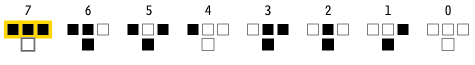
\includegraphics[width=10cm]{images/rule110.png}
       \caption{Rules for Rule 110 \cite{Rule110Img}.}
           \label{fig:Rule110}
\end{figure}

Rule 110 is one of the simplest TC system that is known.
This makes it a relatively easy system to create to demonstrate Turing Completeness as opposed to CGoL.

\subsubsection{Programmable Calculator}\label{subsubsec:ProgCalc}

An entirely different approach to create a program that demonstrates Turing Completeness is to model the behavior of TMs directly.
This means that you create a system that does everything that a TM can do.
Recalling the Church-Turing Thesis (Theorem\ref{thm:CTT}), it must be able to calculate any function.
In a basic sense, this means that the system is capable of:

\begin{itemize}
    \item Reading/Writing memory
    \item Elementary Arithmetic/Logical operations
    \item Conditional Logic
    \item Looping Logic
\end{itemize}

Programmable Calculators meet all of these requirements.
By being able to store values into variables which can be referenced later, it can read/write memory.
Because it is a calculator, it is capable of performing arithmetic operations.
If statements and while loops are sufficient for handling the conditional and looping logic.
A programmable calculator thefore is TC \cite{CalcTC}.
This much simpler approach is clear and follows software engineering design principles.
A simplistic set of steps is outlined below:

\begin{enumerate}
    \item Start by making a basic arithmetic calculator.
    \item Then add the ability to store values into variables.
    \item Afterwards, create functionality for if statements, allowing boolean logic.
    \item Finally, create looping logic with while statements.
\end{enumerate}

\subsubsection{Interpreter for a known Turing Complete language}\label{subsec:InterpreterTC}

Alternatively, to show a programming language is TC, one can create an interpreter for a known TC language.
Many programming languages feature complex grammars and rulesets, which is why TC esoteric programming languages are preferred.
In fact brainfuck, as seen in section \ref{subsubsec:EsotericPL}, is used to demonstrate TC for its concise ruleset \cite{CBfInter,MeepWebsite,MeepGH,PythonBfInt}.

\section{Mathematics}\label{sec:Maths}

In this section, I will take a look at the mathematical system that is most well known for being TC, Lambda Calculus.
This is an abstract form of understanding functions and their capabilities.
It was actually designed by Church, and proven to be TC later on based off the work of Turing and Church by a famous mathematician: Stephen Cole Kleene \cite{LambdaCalcKleene}.

\subsection{Lambda Calculus}\label{subsec:LambdaCalc}

Lambda calculus upon initial inspection seems like a very abstract form of functions and relations within mathematics.
It can be understood to those in Computer Science as a very abstract programming language, and actually forms the basis of Functional Programming Languages \cite{TutLambdaCalc,FuncProgrChap}.

Lambda Calculus is a form of expressing functions in a simple manner that allows for creating any complex system \cite{LambdaCalcRG}.
At its core, it consists of three inductive rules defining what lambda terms are.
Each lambda term is a valid statement in lambda calculus:
\begin{enumerate}
    \item \textit{x}: A \textbf{variable} to represent a character or string.
    This is to be understood as a parameter for functions.
    \item \textit{$\lambda x.M$}: A lambda \textbf{abstraction} that is a function definition.
    This function takes the bound variable \textit{x} as input, and returns the body \textit{M}.
    \item \textit{(M N)}: An \textbf{application} where it applies the function \textit{M} to argument \textit{N}.
\end{enumerate}

\vspace{1cm}
There also exist reduction operations to improve legibility but retain equivalent logical meaning:

\begin{enumerate}
    \item \textit{($\lambda x.M[x]$) $\rightarrow$ ($\lambda y.M[y]$)}: $\alpha$-conversion, which renames the bound variables in the expression.
    This is be used to avoid name collisions.
    \item \textit{(($\lambda x.M$)\textit{N}) $\rightarrow$ ($M[x:=N]$)}: $\beta$-reduction, which replaces bound variables with the argument expression in the body of the abstraction.
    This is used to simplify chained functions being written out.
\end{enumerate}

Parentheses may be used to to disambiguate terms from each other.
This is especially useful when constructing complex applications using lambda calculus \cite{LambdaCalcWiki}.

I will define an equivalent TM to the previously mentioned TM seen in Figure \ref{fig:TM} and in section \ref{subsec:AutomataThy}.
Recall that the goal of the TM was to determine if there are an even or odd number of '1's in a sequence.

We construct the list of Natural Numbers, $\mathbb{N}$, as follows:
\[
    \begin{aligned}
        0 &\equiv \lambda sz.s(z)\\
        1 &\equiv \lambda sz.s(s(z))\\
        2 &\equiv \lambda sz.s(s(s(z)))\\
        &\text{and so on...}\\
    \end{aligned}
\]

Now we construct the ideas of Arithmetic Boolean Logic, and other necessary logical operators.
Treat 'f' as a function and variables as only locally defined to their respective operator \cite{LambdaFuncsList}.
Some notation can be interpreted as SKI combinator calculus \cite{SKICalcWiki}.

% make sure the text is spaced properly in the final version

\[
    \begin{aligned}
        K &:= \lambda xy. x \equiv X(X (X X)) \equiv X' X' X'\\
        S &:= \lambda xyz. (x z) (y z) \equiv X (X (X (X X))) \equiv X K \equiv X' (X' X')\\
        I &:= \lambda x. x \equiv S K S \equiv S K K \equiv X X\\
        Y &:= \lambda g. (\lambda x. g (x x)) (\lambda x. g (x x))\\
        SUCC &:= \lambda nfx. f (n f x)\\
        PRED &:= \lambda n fx. n (\lambda gh. h(g f)) (\lambda u. x) (\lambda u. u)\\
            &\equiv \lambda n. n (\lambda gk. \hspace{0.1cm} ISZERO \hspace{0.1cm} (g \hspace{0.1cm} 1) k \hspace{0.1cm} (PLUS (g \hspace{0.1cm}k) 1))  (\lambda v. 0) 0\\
        PLUS &:= \lambda mnfx. n f (m f x)\\
            &\equiv \lambda mn. n \hspace{0.1cm} SUCC \hspace{0.1cm} m\\
        SUB &:= \lambda mn. n \hspace{0.1cm} PRED \hspace{0.1cm} m\\
    \end{aligned}
\]
\[
    \begin{aligned}
        MULT &:= \lambda mnf. m(n \hspace{0.1cm} f)\\
            &\equiv \lambda mn. m (PLUS \hspace{0.1cm} n) 0\\
        DIV &:= \lambda Y (\lambda gqab. \hspace{0.1cm} LT \hspace{0.1cm} a \hspace{0.1cm} b \hspace{0.1cm} (PAIR \hspace{0.1cm} q \hspace{0.1cm} a)(g \hspace{0.1cm} (SUCC \hspace{0.1cm} q) (SUB \hspace{0.1cm} a \hspace{0.1cm} b) \hspace{0.1cm} b)) 0\\
        MOD &:= \lambda ab. \hspace{0.1cm} CDR \hspace{0.1cm} (DIV \hspace{0.1cm} a \hspace{0.1cm} b)\\
        TRUE &:= \lambda xy. x \equiv K\\
        FALSE &:= \lambda xy. y \equiv 0 \equiv \lambda x. I \equiv K I \equiv S K \equiv X (X X)\\
        NOT &:= \lambda pab. p  b a \equiv \lambda p. p \hspace{0.1cm} FALSE \hspace{0.1cm} TRUE\\
        ISZERO &:= \lambda n. n (\lambda x. \hspace{0.1cm} FALSE) \hspace{0.1cm} TRUE\\
        LT &:= \lambda ab. \hspace{0.1cm} NOT \hspace{0.1cm} (LEQ \hspace{0.1cm} b \hspace{0.1cm} a)\\
        LEQ &:= \lambda mn. \hspace{0.1cm} ISZERO \hspace{0.1cm} (SUB \hspace{0.1cm} n \hspace{0.1cm} m)\\
        PAIR &:= \lambda xyf. f x y\\
        CAR &:= \lambda p. p \hspace{0.1cm} TRUE\\
        CDR &:= \lambda p. p \hspace{0.1cm} FALSE\\
        NIL &:= \lambda x. \hspace{0.1cm} TRUE\\
        NULL &:= \lambda p. p (\lambda xy. \hspace{0.1cm} FALSE)\\
        LENGTH &:= Y \lambda (gcx. \hspace{0.1cm} NULL \hspace{0.1cm} x c (g \hspace{0.1cm} (SUCC \hspace{0.1cm} c) \hspace{0.1cm} (CDR \hspace{0.1cm} x))) 0\\
    \end{aligned}
\]

Now one can combine these lambda functions from a higher abstraction level to perform the operation.

\begin{verbatim}
    Obtain the Length of the List.
    With the list length, subtract 1 from it.
    Take the mod of the result.
    If the new result is 0, then that means it was even.
    If instead it was 1, then it was odd.
\end{verbatim}

Resulting in the following simplified lambda calculus operation:\[MOD \hspace{0.1cm} (SUB \hspace{0.1cm} (LENGTH \hspace{0.1cm} (\textbf{input}) \hspace{0.1cm} 1)) \hspace{0.1cm} 2\]
with \textbf{input} being the input string.
One can expand this result to the above lambda calculus notation, resulting in an extraneously long sequence.
See Figure \ref{fig:OddEvenLambda} for an example of an expanded lambda calculus function that determines if a number is even or odd, i.e. it's cardinality \cite{RedditLambdaCalcPost,RedditLambdaCalcComment}.

\begin{figure}[htb]
    \centering
    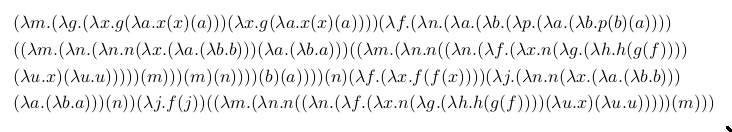
\includegraphics[width=16cm]{Images/oddevenlambda.png}
       \caption{Expanded lambda calculus function to determine the cardinality of a number.}
           \label{fig:OddEvenLambda}
\end{figure}

With the ability to define any calculable function, Lambda Calculus is TC, satisfying the Church-Turing Thesis, Theorem \ref{thm:CTT}.